\medskip
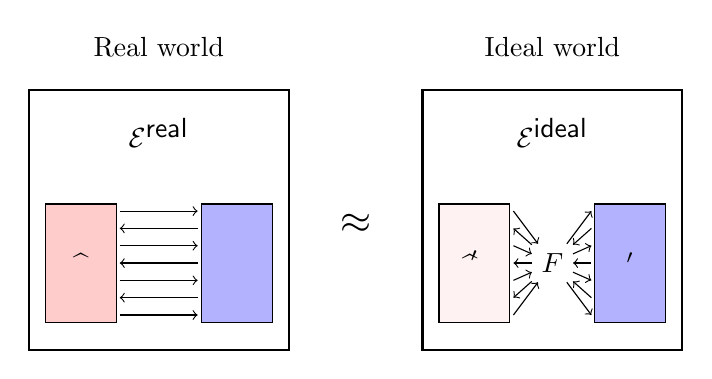
\begin{tikzpicture}
  \begin{scope}[local bounding box=B1, scale=1.1]
    \node at (0, 2.5) {Real world};
    \node[draw, minimum height=1.5cm, minimum width=.9cm, fill=red!20] at (-.9, 0) {$\widehat{\adv}$};
    \node[draw, minimum height=1.5cm, minimum width=.9cm, fill=blue!30] at (.9, 0) {$\cdv$};
    \draw[thick] (-1.5, -1) rectangle (1.5, 2);
    \node at (0, 1.5) {$\mathcal E^{\textsf{real}}$};
    \foreach \i in {0,1,2,3} {
      \draw[->] (-.45, .6 - .4*\i) --(.45, .6 - .4*\i);
    }
    \foreach \i in {0,1,2} {
      \draw[<-] (-.45, .4 - .4*\i) --(.45, .4 - .4*\i);
    }
  \end{scope}
  \node at (2.5, .5) {\Large $\approx$};
  \begin{scope}[local bounding box=B2, xshift=5cm, scale=1.1]
    \node at (0, 2.5) {Ideal world};
    \node[draw, minimum height=1.5cm, minimum width=.9cm, fill=pink!20] at (-.9, 0) {$\widehat{\adv}'$};
    \node[draw, minimum height=1.5cm, minimum width=.9cm, fill=blue!30] at (.9, 0) {$\cdv'$};
    \draw[thick] (-1.5, -1) rectangle (1.5, 2);
    \node at (0, 1.5) {$\mathcal E^{\textsf{ideal}}$};
    \node (F) at (0,0) {$F$};
    \foreach \i in {0,1,2,3} {
      \draw[->] (-.45, .6 - .4*\i) -- (F);
      \draw[->] (F) --(.45, .6 - .4*\i);
    }
    \foreach \i in {0,1,2} {
      \draw[<-] (-.45, .4 - .4*\i) -- (F);
      \draw[<-] (F) -- (.45, .4 - .4*\i);
    }
  \end{scope}
\end{tikzpicture}
\medskip
